\chapter{Methods for Text Classification}\label{chap:nnmethod}

\section{Introduction}

The problem of text classification or text categorization poses the following problem: assign a set of predefined categories to unstructured text that can be used to organize and structure the text appropriately according to the use case. Text classification is an pivotal problem with several applications in biomedicine. For instance, problems such as recognizing reportable cases of cancer from pathology reports, identifying certain phenotypes from clinical notes, performing word sense disambiguation (that is, given a context determine the semantic meaning for the usage of an ambiguous word), and associating medical subject headings (MeSH terms) to scientific articles, can all be reduced to instances of generic text classification problem. Further, text classification can be grouped into two categories namely, (i) multiclass classification (i.e. labels are mutually exclusive) and (ii) multilabel classification where each input can be assigned to more than one label. By definition, it is clear that multiclass classification is a special case of multilabel classification and hence the latter problem becomes more harder to solve than the former.


Traditionally, the problem of text classification is solved by leveraging discriminative models (models that model decision boundary by estimating posterior probabilities) such as support vector machines (SVMs) and logistic regression (LR), only to mention a few, trained on features extracted from the text including bag of words (BOWs)~\cite{sebastiani2005text}. Moreover, it has been observed in the literature that performance gains are achieved with better feature selection techniques, underlying dataset selection, and ensemble approaches~\cite{zhou2012ensemble}. On the other side, better performing models have also be devised by leveraging the field of feature engineering, where the objective is to derive domain specific features that are more relevant and important. For instance, emoticons, exclamations and hashtags form important features for sentiment analysis of Twitter feed~\cite{kiritchenko2014sentiment}. Moreover, especially in the field of biomedicine, exploiting interoperable concept explanations and inter-concept relations from domain specific knowledge base such as unified medical language system (ULMS)\footnote{https://www.nlm.nih.gov/research/umls/} have led performance gains in the accuracy of the underlying models~\cite{yepes2015knowledge}. To this end, models with linear classifiers with ensemble modeling and domain specific feature engineering has the capacity to attain competitive results for the task of text classification.

We perform two experiments for the problem of text classification: (i) Baseline multi-label classification and (ii) Deep learning - specifically CNN and BiLSTM. We illustrate a comparison of the performance of the aforementioned methods in Chapter~\ref{chap: results}. The motivation behind this comparison of employing two techniques is to answer the research question as to which method performs better when we deal with prediction of metadata (Refer RQ4 in Chapter~\ref{chap:intro}).

\section{Baseline Multi-label Classification}\label{MLtranform}
The number of labels (or categories) entails the different kinds of classification problems. For example: if the number of labels $|L| = 2$ then the problem is called binary classification, for $|L| > 2$ labels the problem becomes a multi-class classification. The problem of multi-label classification similarly deals with more than one label, but each label is considered as a different classification problem, but these problems are somewhere related to each other. On the contrary, in a multi-class classification the labels are mutually exclusive~\cite{tsoumakas2007multi}. For instance in a multi-class problem would consider that a scientific publication would only talk about one out of several diseases. Whereas in a multi-label classification the scientific publication might talk about several diseases or none diseases at all. 
In order to use the traditional classification techniques like Random Forest Classifier, Decision trees and so on, the problem needs to be transformed in a way that these techniques can be used. In this project we use three transformation techniques (i) Binary Relevance, (ii) Label Powerset and (iii) Classifier Chains. 
\subsection{Problem Transformations}
Here we briefly describe the problem transformations where traditional classification techniques are modified in such a way that they can be used to perform multi-label classification. 
\paragraph{Binary Relevance (BR)} 
This transformation converts the multi-label problem into a single label problem for each label. Once these problems are solved, a union is taken for all the classes which is the output of the problem. In simpler words, this problem solves a binary classification for each label with any classifier picked as seen in Figure~\ref{fig:BR}. The major disadvantage in this approach is that it does not take label dependencies into account. 
\begin{figure}[!htb]
    \centering
    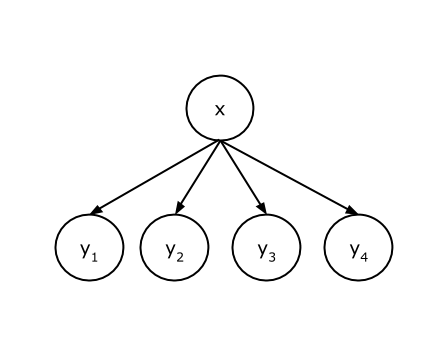
\includegraphics[scale=0.5]{Figures/BinaryRelevance.png}
    \caption{Multi-label problem transformation - Binary Relevance}
    \label{fig:BR}
\end{figure}

\paragraph{Label Powerset (LP)} 
In this problem transformation, a multi-label problem is converted into a single multi-class problem which can take many values. It takes the labels $y_1, y_2, ...., y_n$ (refer Figure~\ref{fig:LP}) and makes several combinations of these labels and solves a multi-class problem for every such combination. This method computes a large space of classes. In total it solves $2^{|L|}$ such problems where $|L|$ is the number of labels. 
\begin{figure}[!htb]
    \centering
    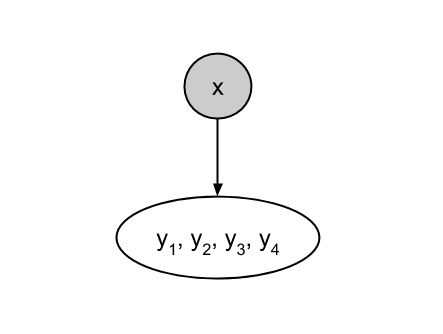
\includegraphics[scale=0.5]{Figures/LabelPowerset.png}
    \caption{Multi-label problem transformation - Label Powerset}
    \label{fig:LP}
\end{figure}

\paragraph{Classifier Chains (CC)}
Classifier chains~\cite{dembczynski2010bayes, read2011classifier} are an improvement in the BR transformation, which takes into account the dependency between the labels if there exists any. Let's say the feature set is: ($x_1, x_2, x_3,....., x_n$) and the set of labels is: ($y_1, y_2, y_3,\ldots, y_n$). The initial feature set is used to predict $y_1$, after that ($x_1, x_2, x_3,\ldots, x_n, y_1$) is used to predict $y_2$. At $n^{th}$ step, feature set ($x_1, x_2, x_3,\ldots, x_n, y_1, y_2, y_3,\ldots, y_{n-1} $) predicts $y_n$ (refer Figure~\ref{fig:CC}). The order of prediction can be tuned in order to get better results. For a large set of labels this method is slow as it takes $n!$ combinations of orderings. 
\begin{figure}[!htb]
    \centering
    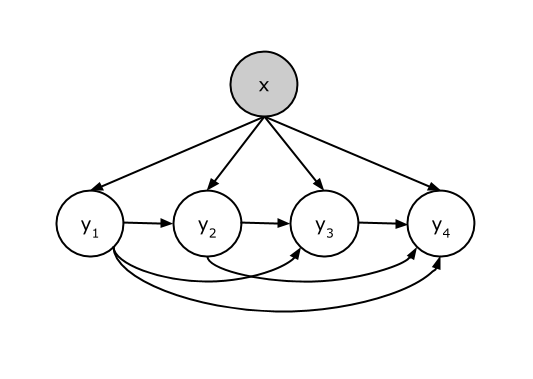
\includegraphics[scale=0.5]{Figures/ClassifierChains.png}
    \caption{Multi-label problem transformation - Classifier Chains}
    \label{fig:CC}
\end{figure}

\subsection{Problem adaptation and Classifiers}
Here we discuss about the adaptation of existing classification algorithms so that they have the ability to perform multi-label classification. Furthermore, we discuss the standard classifiers that have been used. 

\paragraph{Multi-label k Nearest Neighbours (MLkNN)} 
Another adaptation of k nearest neighbours(kNN) for multi-label classification was done by~\cite{zhang2007ml}. In kNN assigns the most commonly occurring neighbours among the calculated k `nearest neighbours'. Whereas in MLkNN, the labels assigned are the most common labels in the neighbourhood of k nearest neighbours. In simpler terms, given a test set, MLkNN uses kNN to find nearest examples and uses Bayesian Inference to predict the labels.

\begin{equation}
 y_{j} = 
\begin{cases}
    1, & \text{if } P(c_{j,x}|y_j = 1)P(y_j = 1) \geq P(c_{j,x}|y_j = 0)P(y_j = 0) \\
    0, & \text{otherwise}
\end{cases}
\end{equation}

(where $c_{j,x} :=$ the number of number of examples present in the neighbourhood of $x$ with $y_j = 1$; Probabilities calculated from the training data)

\paragraph{Decision Trees (DT)}
A decision tree use tree structure perform classification. In such a tree (i) each interior node tests one attribute, (ii) every branch corresponds to an attribute and (iii) each leaf node is the labelled with the class i.e. label/category. A classification using decision tree is presented in Listing~\ref{DT}. It is a strategy for approximating discrete-esteemed capacities that is powerful to load information and equipped for learning disjunctive expressions. The group of decision tree learning calculation incorporates generally utilized calculation, for example, ID3~\cite{quinlan1986induction}, CART~\cite{breiman2017classification} and C4.5~\cite{xiaoliang2009research}. These decision tree learning techniques seek totally expressive speculation space and hence keep away from the troubles of limited theory spaces. Their inductive inclination is an inclination for little trees over substantial trees. 
\begin{lstlisting}[caption = Classification with Decision Trees, label = DT]
Classify(x: instance, node: variable containing a node of DT)
    if node is a classification node then
        return the class of node;
    else
        determine the child of node that match x.
        return Classify(x, child).

\end{lstlisting}



%\todo{still to add brief description about random forest and MLP}
\paragraph{Random Forest}
A random forest is an information build connected to machine learning that grows substantial quantities of random decision trees dissecting sets of factors~\cite{breiman2001random}. This sort of calculation improves the manners in which that advances examine complex information. 

All in all, decision trees are famous for machine learning assignments. In a random forest, engineers build sets of random decision trees to all the more cautiously detach information from information mining, with various connected variable exhibits. One approach to portray the theory behind the random forest is that since the random trees have some cover, specialists can assemble frameworks to consider information needlessly with the different trees and search for patterns and examples that help a given information result. For instance, if five random trees give data on a similar variable from a subset, and four of them concur, the machine learning calculation may use that "dominant part vote" to construct models dependent on probabilities. In a wide range of sorts of machine learning, develops like the random forest can assist mechanical frameworks with drilling down into information and give increasingly modern investigation.

\paragraph{Multi-layer perceptron (MLP)}
Although neural networks are also explained in Section~\ref{section:architecture}, we define MLP here as we use it as a baseline classifier. 
Multilayer feed forward networks, an essential class of neural networks~\cite{haykin1994neural}. Typically, the system comprises of a lot of tangible unit (source hubs) that establish the info layer, one or increasingly concealed layers of computational nodes, and a yield layer of calculation nodes. The input flag engenders through the system in a forward direction, on a layer-by-layer basis. These neural systems are regularly alluded to as multilayer perceptrons (MLPs), which speak to a speculation of the single-layer perceptron. 

Multilayer perceptrons have been connected effectively to tackle some troublesome and differing issues via preparing them in an administered way with a profoundly prominent calculation known as back-engendering calculation. 
A multilayer perceptron has three particular qualities: 
\begin{enumerate}
    \item The model of every neuron in the system incorporates a nonlinear enactment work. 

    \item The system comprise of at least one layers of concealed neurons that are not part of the information or yield of the network. These shrouded neurons empower the system to learn complex assignments by separating dynamically progressively significant highlights from the information design. 

    \item The system displays high degrees of connectivity, determined by the neural connections of the system. 
\end{enumerate}
It is through the mixture of these attributes together with the capacity to gain as a matter of fact through preparing that the multilayer perceptron determines its registering power.

\section{Deep Learning}
The advent of deep neural networks (deep nets) in the last decade or so has led to foundation for generic alternatives to supervised learning, especially for the task of object classification. Deep nets eliminate the laborious process of feature engineering and automatically learn high level representations of input which suites best for the underlying classification problem. Although, the resurgence of deep nets was initially meant for the field of computer vision, recently it has also been applied to natural language processing tasks (NLP)\cite{bengio2003neural, collobert2008unified, mikolov2013distributed} especially through learning distributed representations of words as vectors in high dimensional space. These vectors help the model in guiding elementary tasks such as part-of-speech (POS) tagging and parsing as well as abstract tasks such as text classification and machine translation. Typically, the novel deep learning approaches for text classification rely on architectures based on convolutional neural networks (CNNs) or recurrent neural networks (RNNs)~\cite{young2018recent}. In Figure \ref{fig:dlarch}, you can see a typical deep learning based text classification architecture pipeline.


% . For instance, scientific articles can be filtered by keywords, support tickets can be organized by urgency, tweets on twitter can be organized by sentiments, and so on. Due to the advent of deep learning in the last decade and especially their potential to attain high accuracies has benefited the task of text classification unconditionally. 



\begin{figure}[!htb]
    \centering
    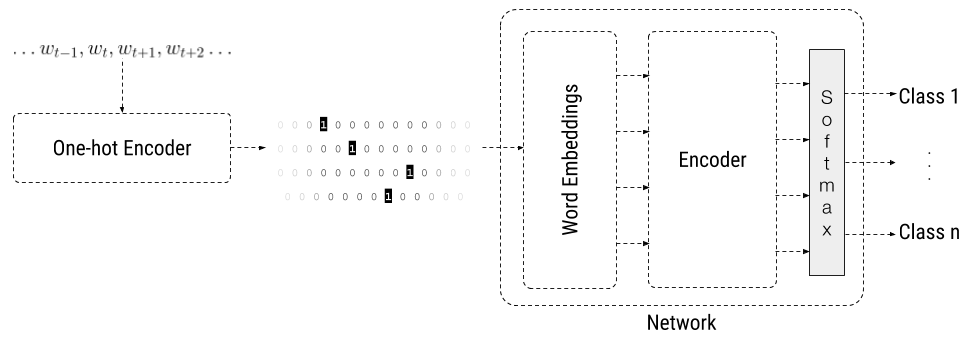
\includegraphics[scale=0.4]{Figures/text-classification-diagram.png}
    \caption{Typical neural network based deep learning architecture for multiclass classification of texts.}
    \label{fig:dlarch}
\end{figure}


Now we unfold each and every component of the architecture in Figure \ref{fig:dlarch}. 

\subsection{Unfolding the architecture}\label{section:architecture}

For an average human, understanding the inherent meaning of the words based on the context they are used, is an easy task. In the same spirit, a deep learning model needs a clever representation of text segments so that it can understand the semantic similarity of related words and also differentiate each word from others. 


\paragraph{One-hot Encoding} Assigning unique, discrete IDs to the word tokens, that is, represented by a \emph{one-hot encoding vector} helps in understanding the model to differentiate between two different words. This in turn has an advantage as neural networks expect vectors as input. Although, this still does not provide any useful information to the model about the relationship between the words and in fact additionally, leads to \emph{sparsity}. 
% This entails that we may need more data in order to obtain meaningful statistical results. 
To state an example, treating words as discrete atomic symbols, for instance, representing a \emph{cat} by \emph{Id100} and \emph{dog} by \emph{Id150} does not provide any meaningful information to the model regarding the relationship that may exist between the two symbols as they are some arbitrary encodings. This amounts to the model leveraging very little of what it has learned about \emph{cats} when it is processing data about \emph{dogs} (such that they are both animals, four-legged, pets, only to mention a few).

\paragraph{Word Embeddings} To overcome the problems regarding sparsity and semantic similarity of related words in one-hot encoding,~\cite{bengio2003neural} developed the concept of word embeddings back in 2003. Despite being introduced before, word embeddings are still relevant today and highly active research domain in deep learning~\cite{bojanowski2017enriching, joulin2017bag, joulin2016fasttext, Peters:2018}. The concept relies on the \emph{Distributional Hypothesis} of J.R. Firth (1957) that states that \emph{``You shall know a word by the company it keeps"}, that is, words that appear in the same contexts share semantic meaning. As we are in the context of neural networks, we are only concerned with predictive methods (i.e. neural probabilistic language models). Predictive models directly try to predict a word from its neighbors in terms of learned small, dense embedding vectors (considered parameters of the model).



A word embedding $\mathcal{W} : \text{words} \rightarrow \mathbb{R}^n$ is a parameterized function that maps words to high dimensional vectors (typically between 200 to 500 dimensions). In other words, it is a dense vector space that forces a fixed dimension on the vector space and forces similar words to appear nearby each other across some dimensions. Typically, the function $\mathcal{W}$ is a look-up table, parameterized by a matrix $\theta$ where each row corresponds to an embedding for a particular word: $\mathcal{W}_{\theta} (w_n) = \theta_n$ (refer Figure \ref{fig:word-embedding-matrix}). $\mathcal{W}$ is initialized randomly by having random row vectors for each word and the model learns to capture meaningful syntactic and semantic regularities in order to perform some task. Word2vec~\cite{mikolov2013distributed} and GloVe~\cite{pennington2014glove} are the two most popular word embedding models to obtain off-the-shelf trainable word embedding matrices. Moreover, word embeddings exhibit an interesting property, namely, it encodes semantic components as linear vector differences. (refer Figure \ref{fig:linear-vector}). 
 

\begin{figure}[!htb]
    \centering
    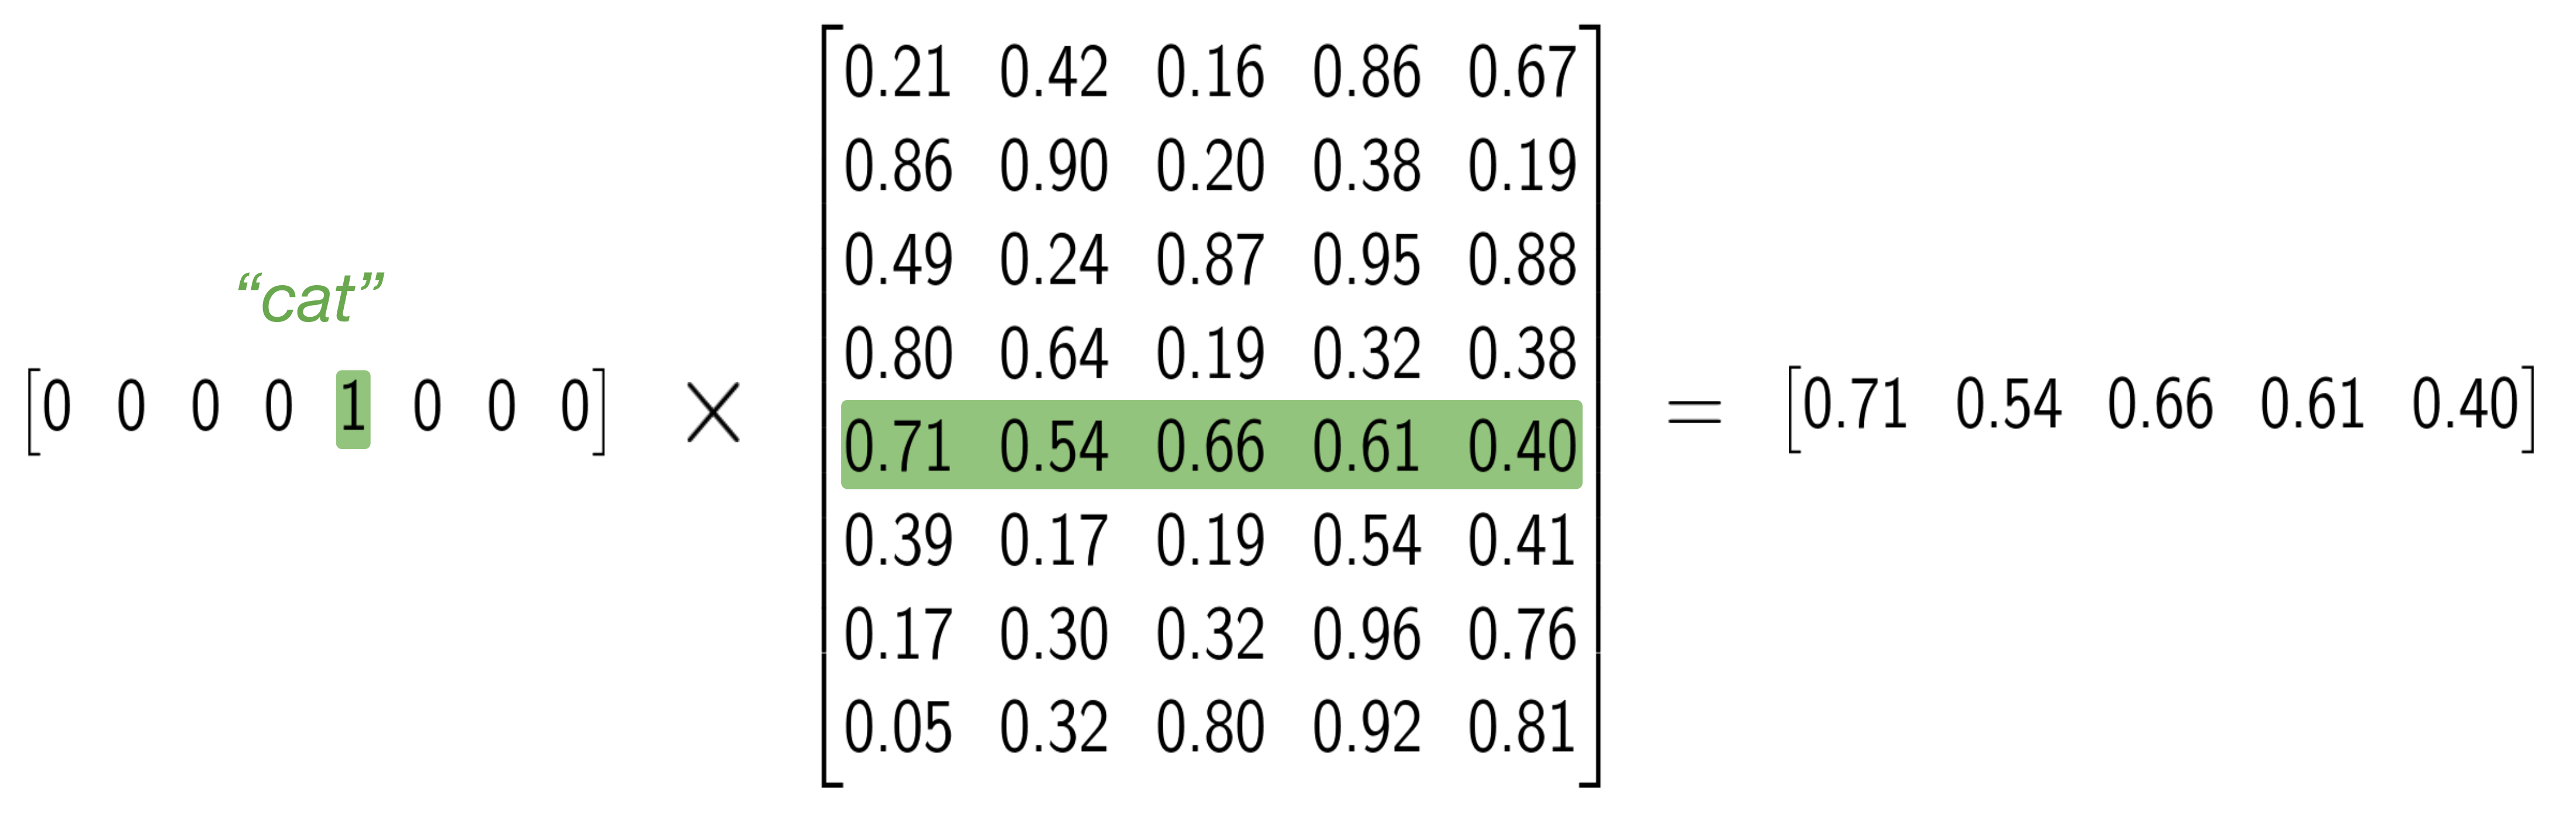
\includegraphics[scale=0.5]{Figures/word-embedding-matrix.png}
    \caption{The figure illustrates how to obtain embedding of a particular word \emph{``cat"} from a word embedding matrix. The one-hot encoding vector of the word \emph{``cat"} is multiplied to the word embedding matrix to obtain the embedding vector for \emph{cat}.}
    \label{fig:word-embedding-matrix}
\end{figure}


\begin{figure}[!htb]
    \centering
    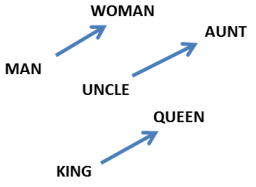
\includegraphics[scale=0.5]{Figures/Mikolov-GenderVecs.png}
    \caption{This figure illustrates the property of word embeddings where linear vector differences between male-female vector is preserved, that is, constant. That is, $\mathcal{W}(``\text{woman}") - \mathcal{W}(``\text{man}") \simeq \mathcal{W}(``\text{aunt}") - \mathcal{W}(``\text{uncle}") \simeq \mathcal{W}(``\text{queen}") - \mathcal{W}(``\text{king}")$ (Image Source~\cite{mikolov2013distributed}).}
    \label{fig:linear-vector}
\end{figure}


\paragraph{Encoder} Once we have the word embedding matrices from the raw text, in order to perform classification tasks, commonly used encoder architectures are convolutional neural networks (CNN) and recurrent neural networks (RNN). Next, we briefly summarize how is the classification task performed using the aforementioned architectures.

\paragraph{Neural Networks}
The neural network (NN) approach is widely used in the machine learning and deep learning algorithms to solve problems with complex, sparse data~\cite{lecun2015deep}. The word `neural' is used because they are loosely inspired by neuroscience. 
%Neural networks are referred to deep feedforward networks or feedforward neural networks.
The goal of such a network is to estimate a function $f^*$.  In a traditional classifier $ y = f^*(\textbf{x})$, it maps the input $\textbf{x}$ to output category $y$. Whereas in the feedforward neural network the model defines a mapping $ y = f(x;\theta)$. It then learns the entries of parameter in $\theta$ which is in-turn best approximation of the function. 
The basic computational unit of a NN is a neuron (refer Figure~\ref{fig:neuron}) which is often referred to as a node or a unit. It receives input from other units or from external source after which it computes an output (see Figure~\ref{fig:vectorinputs}).
\begin{figure}[!htb]
    \centering
    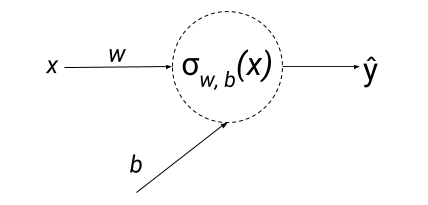
\includegraphics[scale=0.6]{Figures/neuron.png}
    \caption{Typical neuron in a neural network, which can be intuitively thought of a building block of the underlying neural network.}
    \label{fig:neuron}
\end{figure}
\begin{figure}[!htb]
    \centering
    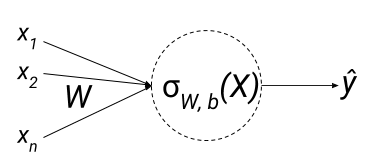
\includegraphics[scale=0.6]{Figures/Vector-Inputs-to-Neuron.png}
    \caption{Vector inputs in the neuron}
    \label{fig:vectorinputs}
\end{figure}
%\todo{include weight vector W in figure}
Each output from this neuron consists of an associated weight ($w$), which is calculated according to the relative importance with respect to other inputs. The node applies a weighted function to the sum of inputs.

The intention behind the network is to learn these set of weights and to be able to control the strength and the influence of these parameters according to the problem that is being solved using the NN approach. We control such an effect of the parameters using an activation function which should be associated to a neuron. Using this function, the node computes the output given a set of inputs. One such activation function is Sigmoid: $\sigma(x) = \frac{1}{1+e^{-x}}$. A parameterized sigmoid function is $\sigma_{w,b}(x) = \frac{1}{1+e^{-wx+b}}$. The advantage of using a non-linear activation function such as sigmoid is that these networks are able to solve non-trivial problems using a relatively smaller number of parameters. 
There are also other types of non-linear activation functions such as: hyperbolic tangent  ($tanh$), Rectified Linear Unit($ReLU$). 

%One limitation of the linear classification like linear regression or logistic regression is that it is not able to detect any correlation between two input variables. NNs are used to perform non-linear classification tasks, 
%For example gradient descent which is a derivative of a linear function gives a smooth function, as nonlinear functions are a generalization of linear functions, 
%see clearly in Figure~\ref{fig:linearclassification} and~\ref{fig:nonlinearclassification}. The neural network which uses a sigmoid function as their activation to perform computations $\sigma(x) = \frac{1}{1+e^{-x}}$, similarly a parameterized sigmoid function is: $\sigma_{w,b}(x) = \frac{1}{1+e^{-wx+b}}$ is shown in Figure~\ref{fig:neuron}. The inputs are given in the form of vectors (refer Figure~\ref{fig:vectorinputs}), if the network contains more than one layers, the composite functions are used to calculate the outputs. Other functions than sigmoid as activation like hyperbolic tangent  ($tanh$), Rectified Linear Unit($ReLU$) etc. 
% \begin{figure}[!htb]
%     \centering
%     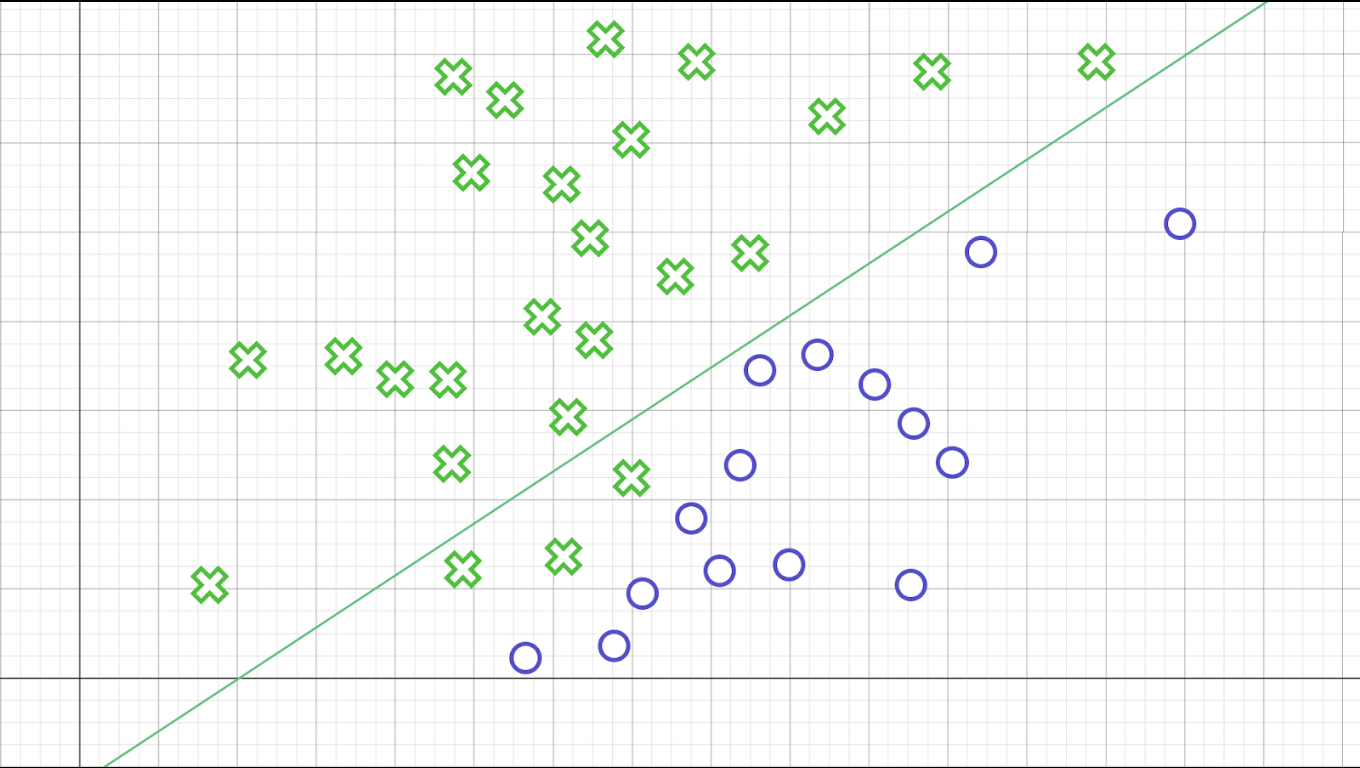
\includegraphics[scale=0.2]{Figures/non-linear_classification.png}
%     \caption{A Linear Classification}
%     \label{fig:linearclassification}
% \end{figure}
% \begin{figure}[!htb]
%     \centering
%     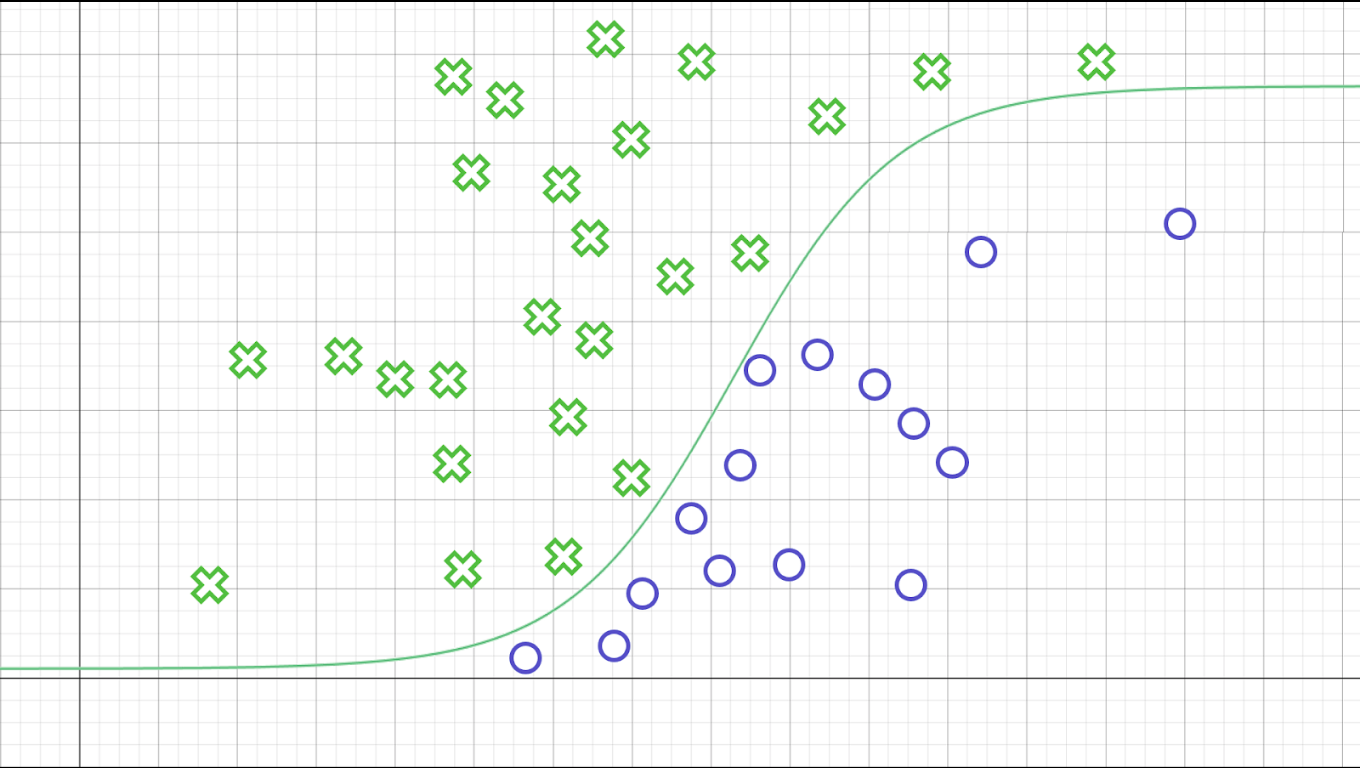
\includegraphics[scale=0.2]{Figures/linear_classification.png}
%     \caption{A Non-linear Classification}
%     \label{fig:nonlinearclassification}
% \end{figure}

In a neural network architecture there are layers which are classified into three type which are mentioned below, all these layers contain nodes which are interconnected to each other in a dense manner also shown in Figure~\ref{fig:nn}:
\begin{itemize}
    \item \textbf{input layer} - this brings in the data into the architecture which is then pass on to the next layer for processing
    \item \textbf{hidden layer(s)} - after the input layers there are a certain number of interconnected layers these can be specified accordingly. Here, the network takes a bunch of weighted set and use an activation function to emit the output.
    \item \textbf{output layer} - last layer of nodes where we get the output.
\end{itemize}
\begin{figure}[!htb]
    \centering
    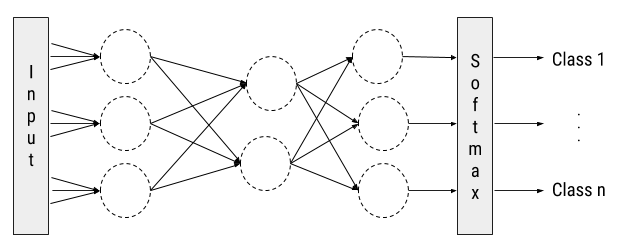
\includegraphics[scale=0.6]{Figures/neural-network.png}
    \caption{A simple neural network architecture for the task of multiclass classification, where the output layer is followed by a softmax layer, that takes outputs from the output layer and converts a distribution of numbers into probabilities.}
    \label{fig:nn}
\end{figure}

While training the neural networks we need to see how every parameter effects on the performance. For this purpose, we calculate the model performance using the function known to us as \emph{loss function}. A loss function is the difference between the model output ($\hat{Y}$) and the given label (Y) for a data point. For instance, one such loss function is mean square error method and is written as, 
\begin{equation}
    L(\hat{Y},Y) = \frac{1}{2n}\sum_{i=1}^{n}(\hat{y}-y)^2
\end{equation}
Given enough hidden units (neurons), a two layered neural network that can approximately imitate any continuous function, over a wide range of activation functions. Although the challenge is to find right values of the parameters given the input data. This is where backpropagation comes into practice. 
We know from high school calculus that for a function $y = f(x)$, $f'(x)$ or $\frac{dy}{dx}$ is an indicative of modifying the value of $x$, where the objective is to minimize $y = f(x)$. That is, in order to reduce $f(x)$, we have to modify $x$ in small steps with an opposite direction of the sign of $f'(x)$--this is gradient descent. Backpropagation is done using gradient descent. The gradients are calculated w.r.t. model parameters for each parameter. The parameters are modified in such a way that the parameters point in that direction where loss is decreasing. The parameters (weights) are modified using the following formulation, where $\eta$ (positive scalar) is a hyperparameter known as learning rate of the neural network model (determines how big a step to take in the direction opposite to the gradient)
\begin{equation}
    w_{n}^{(t+1)} = w_{n}^{(t)} - \eta\frac{dL}{dw_{n}^{(t)}}
    \label{eq:parameterupdate}
\end{equation}

Summarizing from Figure~\ref{fig:oneepoch}, we give the input data $x$ to the neural network, $y$ is the input label of the data and $f_W(x)$ is the model which gives the output $\hat{y}$ ($\hat{y} = f_W(x)$). After this loss is calculated: $L(\hat{y}, y)$. This is the forward propagation. 
Now in the backward  propagation: we calculate gradients $\frac{dL}{dW_{1:n}}$. Then the parameters are updated using the Equation~\ref{eq:parameterupdate} in each epoch. 

\begin{figure}
    \centering
    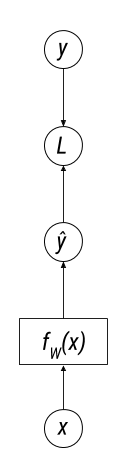
\includegraphics[scale=0.5]{Figures/back-propagation.png}
    \caption{A forward and backward propagation in the neural network.}
    \label{fig:oneepoch}
\end{figure}


\subsubsection{CNN}\label{sec:cnn}
Convolutional neural networks are a special kind of neural networks which employ a grid-like operation. The name ``convolution'' is used because it uses the mathematical operation convolution. In simple words: in a CNN convolution operation is used in at least one of the layers in place of general matrix multiplication~\cite{Goodfellow-et-al-2016}.
They are widely used in the context of images~\cite{krizhevsky2012imagenet} where images are consider 2-D grid of pixels. Although, the architecture can be used if sentences or paragraphs or documents can be represented as matrices or vectors, as it is the case in images. Word embedding matrices typically act as pixel matrices of images in the context of text classification. One of the reasons as to why CNNs are successful is because of its inherent property of keeping a number of copies of the same type of neurons. 
%This helps the model to have numerous neurons, while being able to process large complex models keeping same number of parameters. While writing programs in computer science we tend to write a function and keep calling it later on, the CNNs do a similar thing with the help of these large number of neurons. This in turn makes learning easier and reduces error. 
CNN has been successfully applied in NLP tasks~\cite{dos2014deep, zeng2014relation}. 

From the network point of view, CNN's are essentially several layers of convolutions (refer Figure~\ref{fig:CNN_layer}) stacked upon each other with non-linear activation functions applied to the output of neurons in the same layer. 
\begin{figure}[!htb]
    \centering
    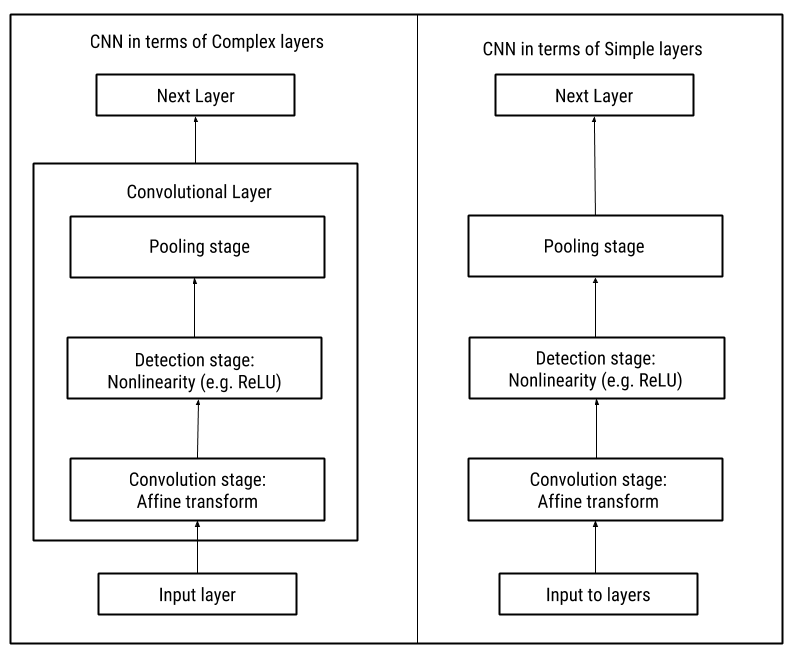
\includegraphics[scale=0.5]{Figures/cnn.png}
    \caption{The figure illustrates the components of a typical convolutional neural network (CNN). The figure in the left views CNN as small number of complex layers, where within each layer a number of operations are applied. While on the right, CNN is viewed as a larger number of simple layers performing elementary operations.}
    \label{fig:CNN_layer}
\end{figure}
A typical layer in a CNN has three stages: (i) convolution operation (refer Figure~\ref{fig:convolution}), (ii) a non-linear activation like rectified linear unit and (iii) a pooling function which lists the set of output with certain statistical explanation of outputs of neighbourhood. These three stages accommodate in the standard feed-forward architecture of linear and non-linear activations. As we can see from Figure~\ref{fig:CNN_layer},
the first stage is linear and the second layer when combined with the third stage form a non-linear activation. 
One of the most used pooling statistics is \emph{max-pooling}. Most commonly, max-pooling is used as a downsampling technique with for instance, say $2 \times 2$ dimension filter and stride equal to 2 , (Figure~\ref{fig:maxpool}), which reduces the representation size and decreases computational and statistical burden on the next layers.



\begin{figure}[!htb]
    % \centering
    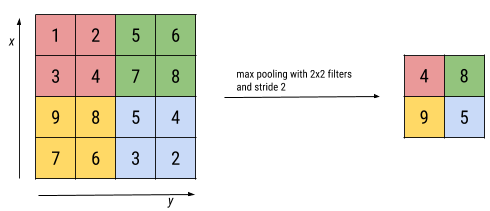
\includegraphics[width=0.6\textwidth, center]{Figures/max-pooling.png}
    \caption{This figure illustrates the operation of max-pooling to summarize the feature maps.}
    \label{fig:maxpool}
\end{figure}
Figure~\ref{fig:convolution} illustrates that convolution is a binary operation that involves two operands namely, some text and a predefined kernel or filter, both of which are represented as matrices containing real numbers.
\begin{figure}[!htb]
    % \centering
    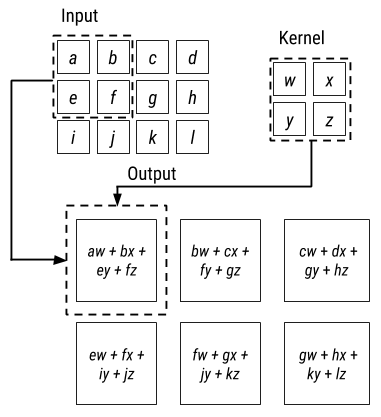
\includegraphics[width=0.6\textwidth, center]{Figures/convolution.png}
    \caption{This figure illustrates the operation of convolution on a 2D image. Boxes and arrows are drawn which indicate how the convolution takes place when the kernel/filter is applied to the upper-left region of the input.}
    \label{fig:convolution}
\end{figure}
Typically, the matrix representation of text comprises of the word vectors of tokens that constitute it, that is, the word embedding matrix. The objective of the kernel is to operate on all contiguous segments of the text using a sliding window and produce real numbers of cardinality that is equal to the number of contiguous segments (in text). This sequence of real numbers is called a feature map and is associated with a particular kernel being used to compute it. Generally, different kernels produce different feature maps that can be used as features for the task of text classification. The feature maps are then fed into a non-linear activation function as input, typically, softmax (function that takes $l$ real values as input and normalizes it into a probability distribution consisting of $l$ probabilities)   in our use case that outputs class or label probability estimates. The main idea here is to learn the matrix representations of kernels that in turn provide better feature maps, which optimizes the objective function efficiently. The learning takes place by predicting labels for training data and make adequate modifications to the kernel matrix through the back propagation algorithm that minimizes the loss function, that is, minimizes the conditional log-likelihood of training data. In the aforementioned abstract elucidation, we have omitted the technical details pertaining to CNNs like mathematical definition of convolution, the objective function and regularization. For the sake of completeness, we discuss these points in detail in the next section.

\paragraph{CNN Model Description}
The architecture of a CNN model with two layers including one convolution layer and a densely connected output layer is depicted in Figure~\ref{fig:Cnn_one_layer}.
\begin{figure}[!htb]
    % \centering
    % 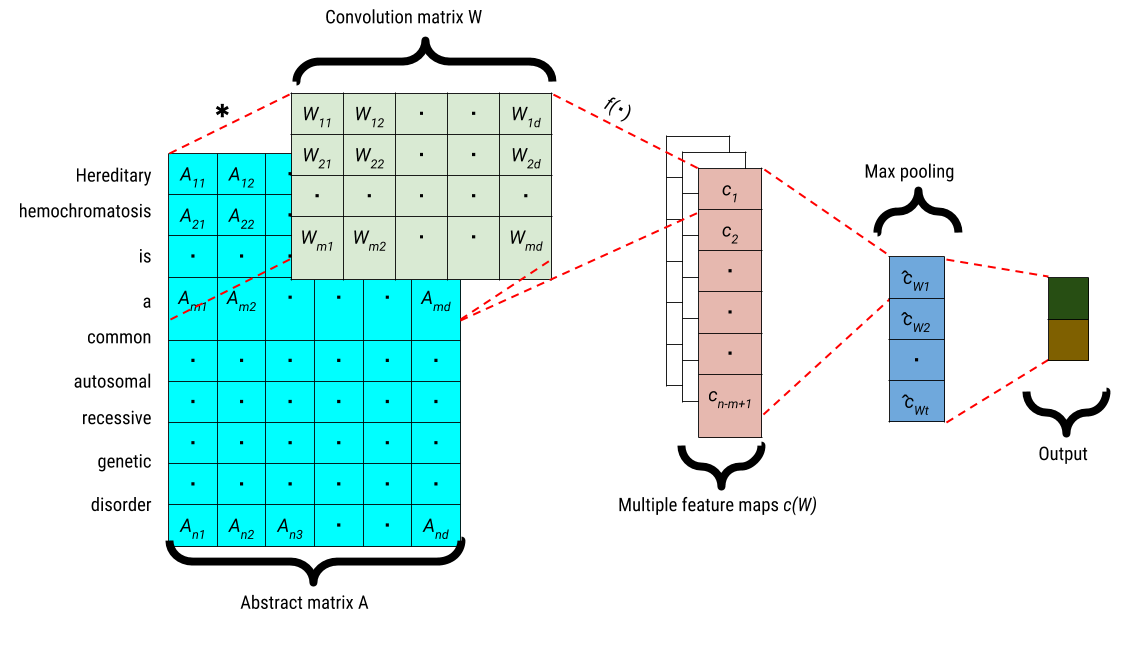
\includegraphics[scale=0.45]{Figures/cnn-model-example.png}
    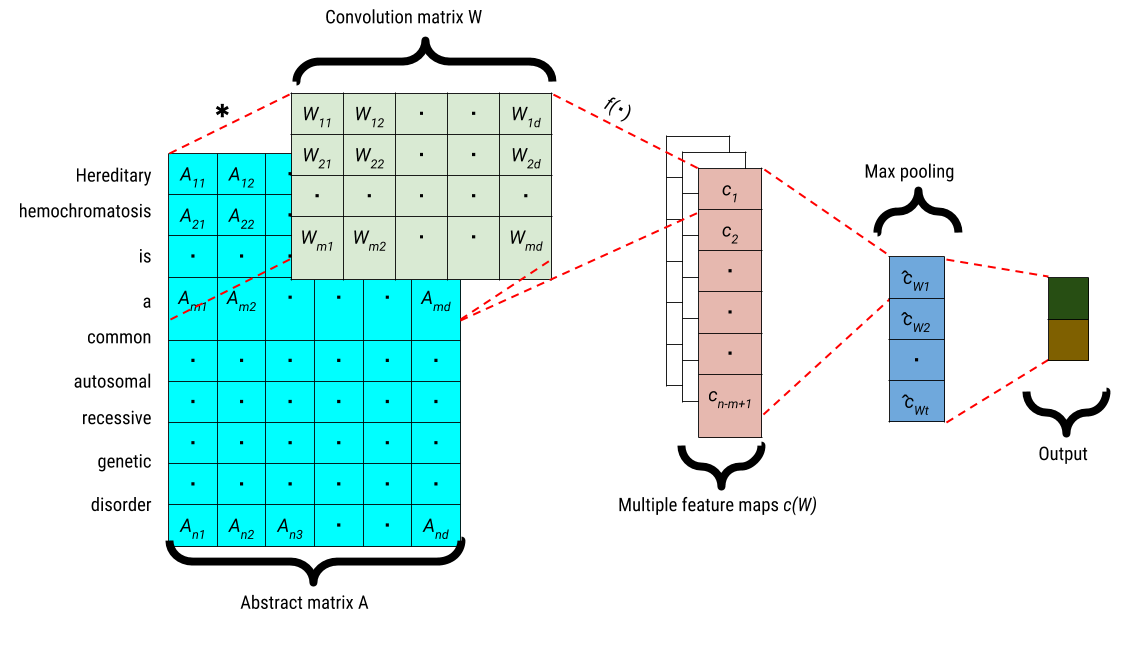
\includegraphics[width=1\textwidth,left]{Figures/cnn-model-example.png}
    \caption{This figure illustrates a CNN with one convolution layer that is precisely used in the experimental setup in this thesis in the context of biomedical abstracts.}
    \label{fig:Cnn_one_layer}
\end{figure}
The basic component of the model is the word vector $\mathbf{x} \in \mathbb{R}^d$, where $d$ is the dimension of the word vectors. An abstract is represented as a matrix $A \in \mathbb{R}^{n \times d}$, where $n$ is the number of words in it. As mentioned earlier in the section~\ref{section:architecture}, each row corresponds to the word vector for the corresponding token or word. For the sake of brevity, we assume that the ground truth (label) for the abstract is $y \in \mathbb{R}^2$ such that $y_2 = 1$ and $y_1 = 0$ ($y_2 = 0$ and $y_1 = 1$) when we are training on a positive (negative) instance. This precisely aligns with the Figure~\ref{fig:Cnn_one_layer} with two output nodes of the final layer for the two classes (positive or negative) for each binary classifier. In this project we perform classification for 48 classes. 
%\todo{mention the number of classes for which the problem is solved !! was it 26 ?}.

We define a kernel $\mathbf{W} \in \mathbb{R}^{m \times d}$, where $m$ is the length of the sliding window. The two-dimensional convolution operation $\mathbf{*}$ can now be defined as follows,

\begin{center}
\[\mathbf{W} * A_{j:j+m-1} = \sum_{i=j}^{j+m-1} \sum_{k=0}^{d-1} \mathbf{W}_{i,k} A_{i,k}.
\]
\end{center}

Next, by using a non-linear function $f(\cdot)$, we map a window of length $m$ to a real number $c_j \in \mathbb{R}$ as 

\[c_j = f(\mathbf{W} * A_{i, j:j+m-1} + b),
\]
 
 where $b \in \mathbb{R}$ is the bias. In this thesis, $f(\cdot)$ is a Rectified Linear Unit (ReLU)~\cite{glorot2011deep, nair2010rectified}. We get the following feature map after convolving over the whole abstract,

 \[\mathbf{c(W)} = [c_1, \ldots, c_{n-m+1}].\]

 Further, to overcome the problem of abstracts of varying lengths, we perform the statistical operation of max-pooling~\cite{zhou1988image} (see also Figure~\ref{fig:maxpool})

 \[\widehat{c_{\mathbf{W}}} = \max_{i} \mathbf{c(W)}_i,\]

 that yields a feature $\widehat{c_{\mathbf{W}}}$ associated to the feature map generated by $\mathbf{W}$. Suppose that we want to learn $t$ kernels $\mathbf{W}^1, \ldots, \mathbf{W}^t$, to obtain multiple features maps. This leads to $t$ single max-pooled features which can be represented as follows,

 \[ \mathbf{\widehat{c_{\mathcal{W}}}} = [\mathbf{\widehat{c_{\mathbf{W}^1}}}, \ldots, \mathbf{\widehat{c_{\mathbf{W}^t}}}],
 \]

 where $\mathcal{W} = \{\mathbf{W}^1, \ldots, \mathbf{W}^t\}$. After this, finally we add a softmax layer. The parameters of the softmax layer $\mathbf{V} \in \mathbb{R}^2 \times t$ and $b^{V} \in \mathbb{R}^2$ with weighted inputs 

 \[y_j = \mathbf{V}_j \mathbf{\widehat{c_{\mathcal{W}}}} + b^{V}_j\]

and output label probability estimates as

\[P(y_j = 1 | A, \mathcal{W}, b, \mathbf{V}, b^{V}) = \frac{e^{y_j}}{\sum_i e^{y_i}},\]

where $\mathbf{V}_j$ $b^{V}_j$ are the $j^{th}$ row and $j^{th}$ element of $\mathbf{V}$ and $b^{V}$ respectively. $y_j$ is the $j^{th}$ label for the abstract corresponding to matrix $A$. 

If $\mathcal{A}$ is the set of training abstract matrices, then in order to learn each binary classifier, we minimize the following loss/objective function

\[- \sum_{A \in \mathcal{A}} \log(P(y_j^A = 1 | A, \mathcal{W}, b, \mathbf{V}, b^{V})),\]

where $j=1$ or $j=2$ depending upon the positive or negative training instance and $y^A$ is the ground truth label for the abstract represented by $A$. The parameters of CNN, that is $(\mathcal{W}, b, \mathbf{V}, b^{V})$ that minimize the loss function are modified by employing the back propagation algorithm with stochastic gradient descent approach. 

As a regularization term so that the model doesn't overfit, we use dropout~\cite{srivastava2014dropout}. More specifically, instead of feeding $y_j$ to the softmax function during training, we actually feed 

\[ \widehat{y_{j}} = \mathbf{V}_j( \mathbf{\widehat{c_{\mathcal{W}}}} \circ \mathbf{s}) + b^{V}_j,
\]
 
where $\circ$ refers to hadamard product (element-wise multiplication) and $\mathbf{s} \in \{0,1\}^t$ is generated with each element $s_i$ drawn from the Bernoulli distribution with parameter $p$ set to $0.2$. In layman terms, this means that the gradients are backpropagated only through those neurons where $s_i = 1$. 

% Note that, while testing the model, we downscale the weights $\mathbf{V}$ such that 

% \[y_j = p\mathbf{V}_j \mathbf{\widehat{c_{\mathcal{W}}}} + b^{V}_j.\]

% This operation is essential because during training, only $80\%$ of the edges are active, that is obviously not true when we test the model. 


\subsubsection{RNN}
Recurrent neural networks~\cite{rumelhart1988learning} are used for processing sequential data. Since language is sequential in nature because when we deal with natural language there is context required for predicting what comes next. RNNs are widely used in natural language models as it used to process sequential data.
As a human being, every time when we try to solve something we don't reboot the brain, instead we remember things and try to build on from that. The traditional neural networks cannot have persistence they always re-learn for scratch unlike human brain, for example if we want to predict what word would come next in the sentence or when we want to do a prediction of the next term in the sequence. In such cases we need the information of what happened previously stored in the network, the RNNs are able to do such computations because they have loops in the network as can be seen in the Figure~\ref{fig:rnnarch}~\cite{chung2015recurrent}. They try to keep track of the information that was learnt previously. 
%Whereas when we deal with natural language there is context required for predicting what comes next, sometimes there is a difference between that there is a big difference between the relevant information and the point where it is needed. 
RNNs do not always perform best when handling ``long term dependencies''~\cite{bengio1994learning}. To overcome this problem, Long Short Term Memory networks (LSTMs) were introduced by~\cite{hochreiter1997long} that are a special kind RNNs which can handle learning the long term dependencies. 

\paragraph{RNN Model Description}
Figure~\ref{fig:rnnarch} introduces the RNN architecture where the input $x_t$ is fed is a hidden layer at time step $t$. 
\begin{figure}
    \centering
    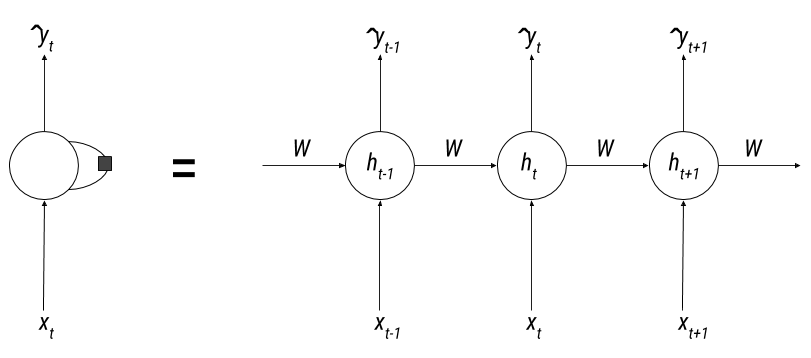
\includegraphics[scale=0.5]{Figures/rnn_figure_1.png}
    \caption{Recurrent Neural Network}
    \label{fig:rnnarch}
\end{figure}
Here, each layer consists of neurons, where each neuron performs a linear matrix operation on its corresponding input which is followed by a non-linear operation. At each time step, the output of the previous step along with the next word vector in the abstract are inputs to the hidden layer that yields $\widehat{y}$ as output and features $h_t$. The inputs and outputs to each neuron in the RNN can be described as follows,

\begin{equation}
\begin{aligned}
	h_t = W f(h_{t-1}) + W^{(hx)}x_t
\end{aligned}
\end{equation}

\begin{equation}
\begin{aligned}
	\widehat{y} = W^{(S)}f(h_{t})
\end{aligned}
\end{equation}

Next, we mention the details associated with each parameter in the network:

\begin{itemize}
	\item Suppose the abstract is of $n$ words in total. Then $x_1, \ldots, x_n$ is the word vectors corresponding to the words of the abstract.

	\item $h_t = \sigma(W^{hh}h_{t-1} + W^{hx}x_t)$ corresponds to the hidden layer features at a particular time step $t$. Here $x_t \in \mathbb{R}^d$ is the input word vector at time step $t$. $W^{hx} \in \mathbb{R}^{D_h \times d}$ and $W^{hh} \in \mathbb{R}^{D_h \times D_h}$ are the weight matrices used to condition input word vector $x_t$ and output of previous time step $h_{t-1}$ respectively.

	\item $\widehat{y}_t = \text{softmax}(W^{(S)} h_t)$ corresponds to the output probability estimates over the vocabulary at each time step $t$. $W^{(S)} \in \mathbb{R}^{|V| \times D_h}$ and $\widehat{y} \in \mathbb{R}^{|V|}$ where $|V|$ is vocabulary.


\end{itemize}

The RNNs are trained using an extension of back propagation algorithm known as back propagation through time (BPPT) algorithm. More specifically, it begins by unfolding the RNN in time: (i) each timestep has one input, one copy of the network (every copy of the network shares the same parameters), and one output, (ii) errors are calculated and accumulated for each timestep, and (iii) the network is rolled back up and the weights are updated.  Then the back propagation algorithm is applied traditionally. The main disadvantage of RNNs is that they can not capture long-term dependencies due to vanishing/exploding gradients during backpropagation. More specifically, if the weights of the word embedding matrix which is input to the RNN are small, it can lead to a vanishing gradients where the gradient signal is so weak that the learning is slow or stops altogether. Conversely, if the weights are large, it can lead to very strong gradient signal that causes the learning to diverge, that is, exploding gradients.

To overcome the problem of long-term dependencies, LSTM was developed, that is, to gain more persistent memory. The mathematical formulation of the LSTM unit is described below,

\begin{equation}
\begin{aligned}
	i^{(t)} = \sigma(W^{(i)}x_t + U^{(i)}h_{t-1}) && \text{(Input \ Gate)} \\
	f^{(t)} = \sigma(W^{(f)}x_t + U^{(f)}h_{t-1}) && \text{(Forget \ Gate)} \\
	o_t = \sigma(W^{(o)}x_t + U^{(o)}h_{t-1}) && \text{(Output \ Gate)} \\
	\widetilde{c}^{(t)} = \text{tanh}(W^{(c)}x_t + U^{(c)}h_{t-1}) && \text{(New \ Memory \ cell)} \\
	c^{(t)} = f^{(t)} \circ \widetilde{c}^{(t-1)} + i^{(t)} \circ \widetilde{c}^{(t)} && \text{(Final \ memory \ cell)} \\
	h^{(t)} = o_t \circ \tanh(c^{(t)})
\end{aligned}
\end{equation}


%\todo{Draw Figure LSTM unit explaining gates}
\begin{figure}[!htb]
    \centering
    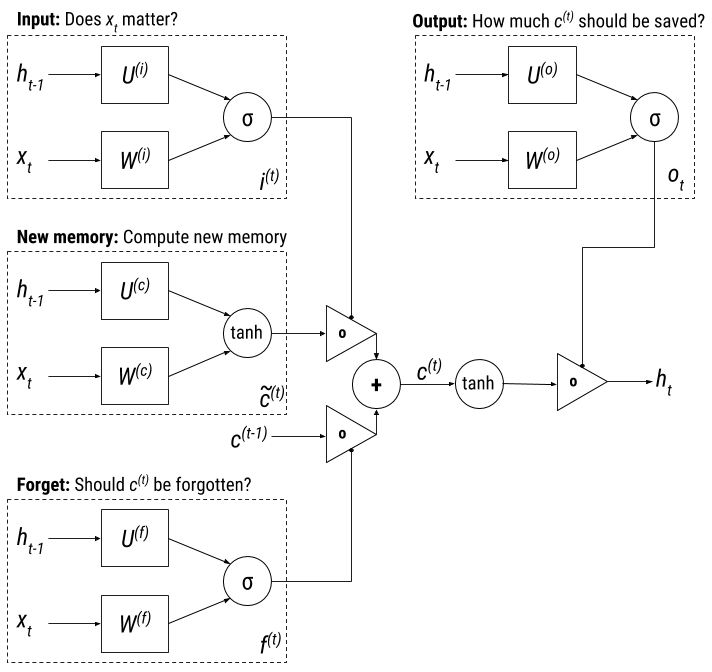
\includegraphics[scale=0.55]{Figures/lstm-unit.png}
    \caption{The detailed internals of a LSTM unit}
    \label{fig:lstmunit}
\end{figure}

Finally, we explain the structure and the intuition behind LSTM units below:

\begin{itemize}
	\item \textbf{New memory generation: }It is the consolidation of a new input word vector $x_t$ with the past hidden state $h_{t-1}$. From the model point of view, this gate cooks the recipe of summarizing the new input in the light of contextual past.

	\item \textbf{Input Gate: }The new memory cell generates new memory blindly without even bothering whether the new input is important or not -- the objective of the input gate is to determine the importance to the new input by using it and the past hidden state. Hence, it is used to gate the new memory and produces $i^{(t)}$ which indicates information.

	\item \textbf{Forget Gate: }The forget gate is analogous to input gate in the sense that it makes an assessment on the usefulness of the past memory cell that is used for the computation of current memory cell. Thus, it looks at the input and the past hidden state and produces $f^{(t)}$.

	\item \textbf{Final memory generation: }Both the input gate and the forget gate act as an advisory to final memory cell, that is, whether to forget past memory or gate new memory respectively. The final memory cell then sums these results to produce the final memory $c^{(t)}$.

	\item \textbf{Output Gate: } Its objective to the separate final memory $c^{(t)}$ from the hidden state. $c^{(t)}$ might not necessarily contain only relevant information all the time that is required to be saved by the hidden state. Moreover, as hidden states are used in every gate of an LSTM unit, the output gate makes an assessment regarding the importance of the information to be stored in the hidden state $h_t$. This produces $o_t$ and this is to gate the point-wise $tanh$ of the memory.
\end{itemize}

The bi-directional version of RNN or LSTM, at each time-step $t$, maintains two hidden layers, one for left-to-right propagation and another for right-to-left propagation. Clearly, this consumes two times as much memory as RNNs. The final output $\widehat{y_t}$ is obtained by combining the scores computed by both the hidden states.


